\documentclass[English]{article}
%^ Start of document
\usepackage{biblatex} %Imports biblatex package
\usepackage{graphicx} % Required for inserting images
\usepackage{authblk}
\usepackage[colorlinks=true, urlcolor=blue, linkcolor=red]{hyperref}
\usepackage{subfig}
\usepackage{float}
\usepackage{tabularx}
\usepackage{multirow}
\usepackage[paperheight=6in,
   paperwidth=5in,
   top=10mm,
   bottom=20mm,
   left=10mm,
   right=10mm]{geometry}
\usepackage{moresize}
\usepackage{tikz}
\usepackage{xcolor}
\usepackage{physics}
\usepackage{amssymb}
\usepackage{mathrsfs}
\usepackage{amsmath}
\usepackage{ragged2e}
\usepackage{comment}
\usepackage{xcolor}
\addbibresource{ElectroHW1.bib}
\begin{document}

\title{Classical Electrodynamics HW 1}

\author[1]{Zachary Tullier}
\affil[1]{Student\\Physics Department\\ University of Houston - Clear Lake \\Houston, Texas\\U.S}

\maketitle


\section{Textbook Question 1.1} \label{section1}
    \underline{Question : }
    \newline Use Gauss’s theorem [and (1.21) if necessary] to prove the following:
    \begin{enumerate}
        \item [a)] Any excess charge placed on a conductor must lie entirely on its surface. (A conductor by definition contains charges capable of moving freely under the action of applied electric fields.)
        \item [b)] A closed, hollow conductor shields its interior from fields due to charges out-side, but does not shield its exterior from the fields due to charges placed inside it.
        \item [c)] The electric field at the surface of a conductor is normal to the surface and has a magnitude (o/¢), where o is the charge density per unit area on the surface.
    \end{enumerate}

    \newpage
    \underline{Question 1, Section a) Answer: }
    \newline 
    \newline Assumptions
    \begin{itemize}
        \item Perfect conductor; therefore charges are perfectly free to move within the conductor
        \item A conductor by definition contains charges capable of moving freely under the action of applied electric fields
        \item The charges that are located are in static equilibrium; therefore there is no electric field in the volume where the free charges exist. The charges at the surface cannot leave the surface; therefore there is only electric field at the surface, normal to that surface. Therefore any tangential force from the electric field is zero. 
        \item If the surface charge is positive, the electric field is outward, and vice versa.     
    \end{itemize}
    
    \begin{figure}[H]
        \centering
        {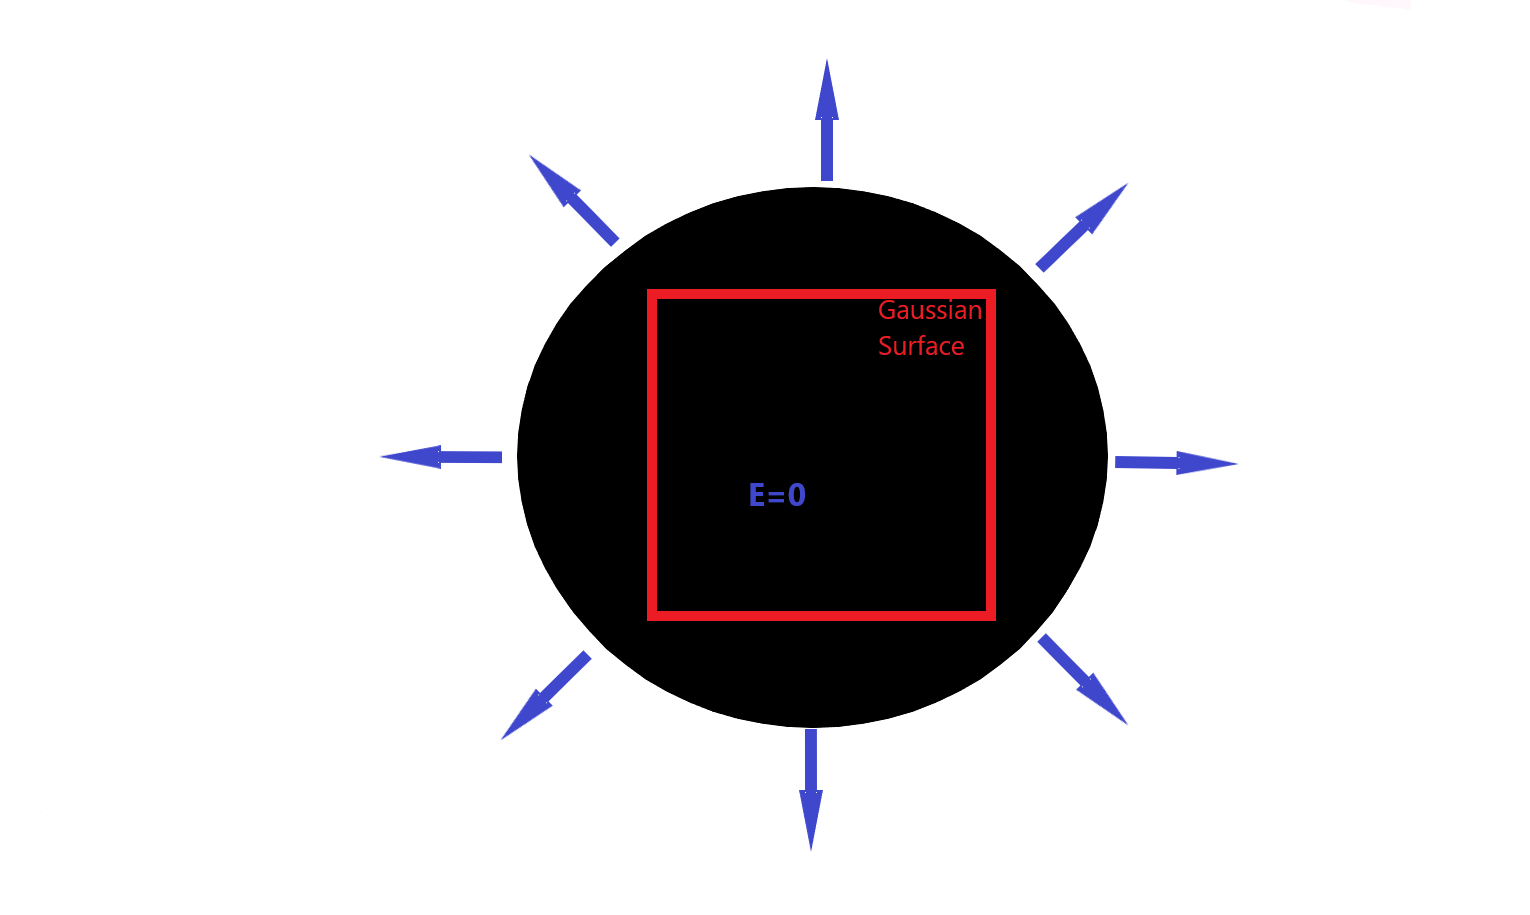
\includegraphics[width=0.4\textwidth]{Images/sphere.png}\label{fig:f1}}
        \caption{Closed Gaussian Surface within the conductor}
    \end{figure}

    Using Gauss's Law
    \begin{equation} \label{eq: 1-1}
        \nabla \cdot \vec{E} = \frac{\rho}{\epsilon_0}
    \end{equation}

    Take integral for an arbitrarily shaped 3D solid conductor with excess charge 
    \begin{equation} \label{eq: 1-2}
        \int_V \nabla \cdot \vec{E} d^3x = \int_V \frac{\rho}{\epsilon_0} dV
    \end{equation}

    Using Divergence Theorem
    \begin{equation} \label{eq: 1-3}
        \int_V \nabla \cdot A d^3x = \int_S A \cdot n da
    \end{equation}

    Substitute equation \ref{eq: 1-3} into equation \ref{eq: 1-2}
    \begin{equation} \label{eq: 1-4}
        \int_S \vec{E} \cdot n da = \int_V \frac{\rho}{\epsilon_0} dV
    \end{equation}

    Evaluate Integral on right
    \begin{equation} \label{eq: 1-5}
        \int_S \vec{E} \cdot n da = \sum_i \frac{q_i}{\epsilon_0}
        \\\int_S \vec{E} \cdot n da = 0
    \end{equation}

    Physically, we can understand this as the net free charges mutually repelling each other and accelerating away from each other until they hit the surface. The only boundary for mutually repelling, freely moving charges is the surface of the conductor; therefore, they all reside on the surface.

    \newpage
    \underline{Question 1, Section b) Answer: }
    \newline \newline Assumptions
    \begin{itemize}
        \item The hollow sphere is connected to ground so that when the external electric field is applied, the charge density of the conductor becomes whatever is opposite of the external electric field.
        \item Perfect conductor; therefore charges are perfectly free to move within the conductor
        \item A conductor by definition contains charges capable of moving freely under the action of applied electric fields
    \end{itemize}
    
    First we make a closed Gaussian surface completely within the the hollow conducting shell and place charge outside of the shell
    \begin{figure}[H]
        \centering
        {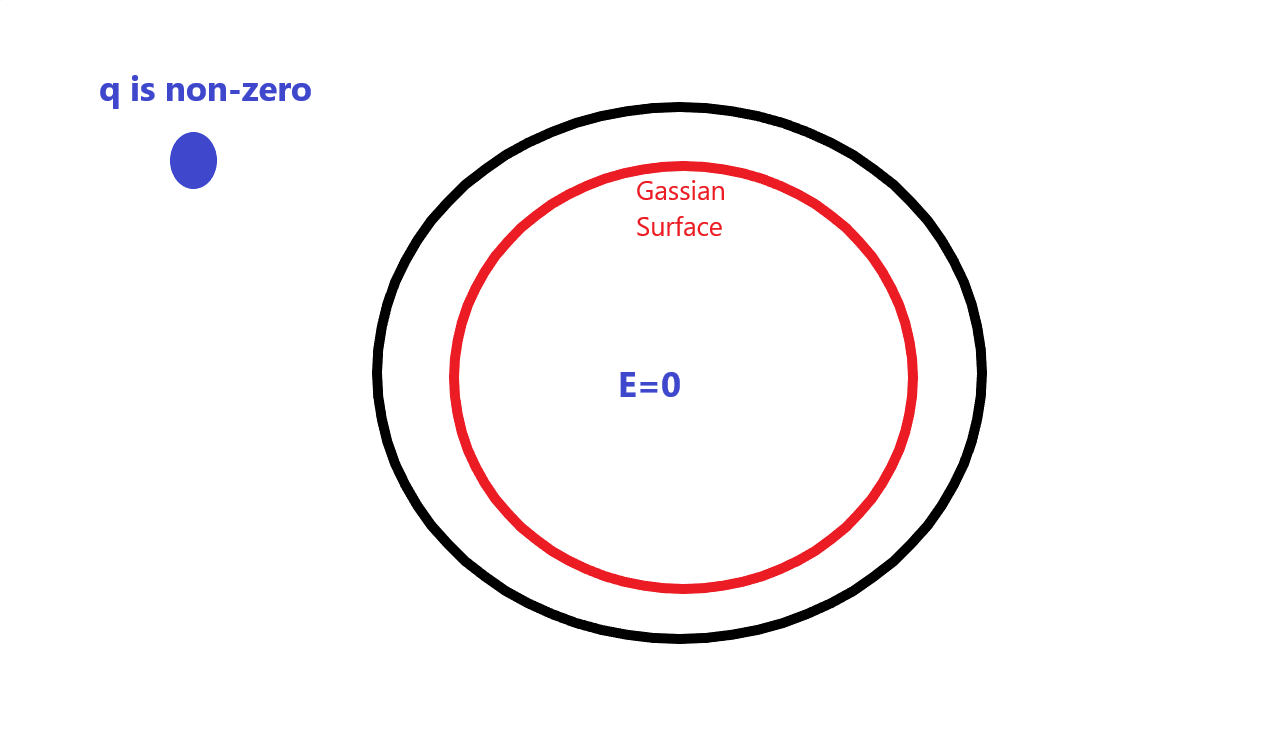
\includegraphics[width=0.4\textwidth]{Images/hollowsphereoutside.png}\label{fig:f2}}
        \caption{Closed Gaussian Surface within the hollow shell conductor with external electric field}
    \end{figure}
    
    Using Gauss's Law in integral form
    \begin{equation} \label{eq: 1-6}
        \oint_S \vec{E} \cdot n da = \frac{\int_V \rho_q(x) d^3 x}{\epsilon_0}
    \end{equation}
    
    Within the gaussian surface there are no charges ($q=0$); therefore:
    \begin{equation} \label{eq: 1-7}
        \oint_S \vec{E} \cdot n da = 0
    \end{equation}

    If the Gaussian surface was chosen to be mostly along the hollow shells inner surface ($\oint_A \vec{E} \cdot n da$) and the rest of the gaussian surface ($\oint_B \vec{E} \cdot n da$) then we would get
    \begin{equation} \label{eq: 1-8}
        \oint_A \vec{E} \cdot n da + \oint_B \vec{E} \cdot n da = 0
    \end{equation}

    Since $\oint_A \vec{E} \cdot n da = 0$ then, $\oint_B \vec{E} \cdot n da = 0$; Therefore, any external field will not have any effect on the inner surface of the conductor, let alone the hollow interior. 

    Now we consider the same conductor with a charge on the inside

    \begin{figure}[H]
        \centering
        {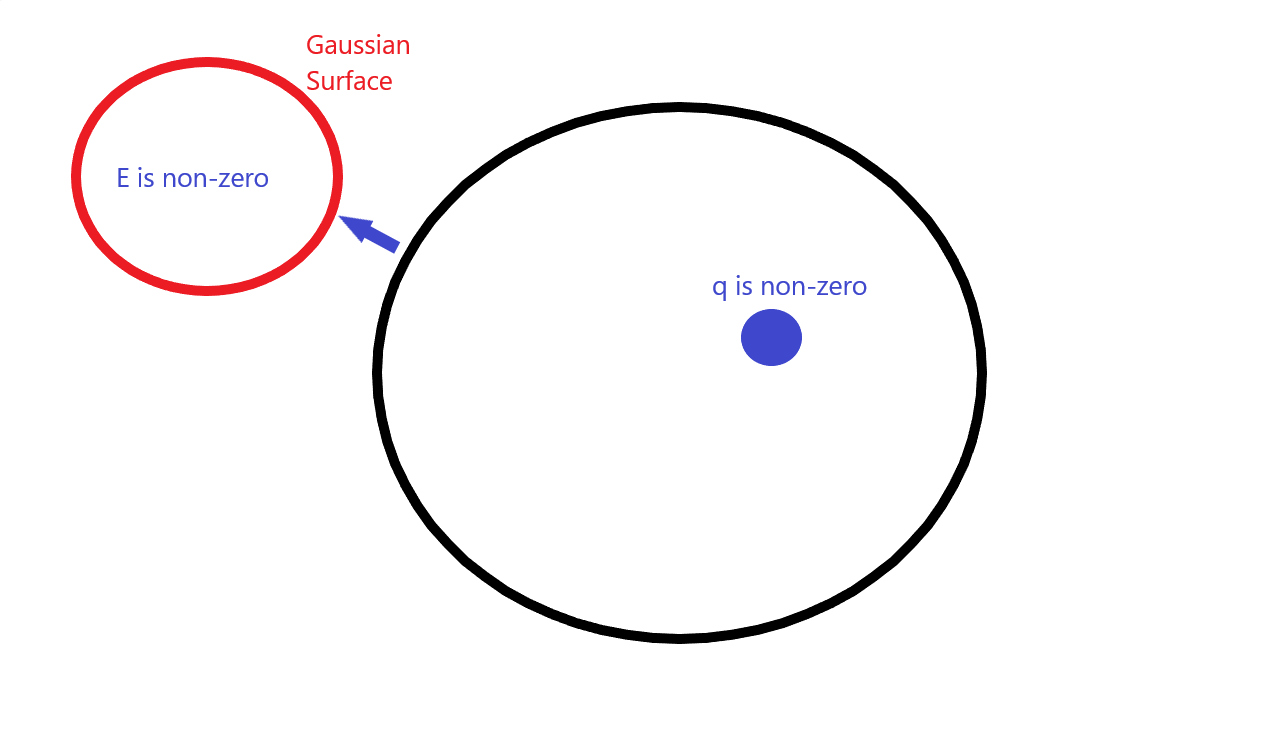
\includegraphics[width=0.4\textwidth]{Images/hollowsphereinside.png}\label{fig:f3}}
        \caption{Closed Gaussian Surface within the hollow shell conductor with internal electric field}
    \end{figure}

    Using Gauss's Law in integral form (Reference equation \ref{eq: 1-6})
    \begin{gather*}
        \oint_S \vec{E} \cdot n da = \frac{\int_V \rho_q(x) d^3 x}{\epsilon_0}
    \end{gather*}
        
    The charge on the outer surface of the hollow conducting shell induced by the charge within will generate an electric field such that:
    \begin{equation}
        \oint_S \vec{E} \cdot n da \neq 0 
    \end{equation}

    \newpage
    \underline{Question 1, Section c) Answer: }
    \newline \newline Assumptions
    \begin{itemize}
        \item Perfect conductor; therefore charges are perfectly free to move within the conductor
        \item A conductor by definition contains charges capable of moving freely under the action of applied electric fields
        \item The charges that are located are in static equilibrium; therefore there is no electric field in the volume where the free charges exist. The charges at the surface cannot leave the surface; therefore there is only electric field at the surface, normal to that surface. Therefore any tangential force from the electric field is zero. 
        \item If the surface charge is positive, the electric field is outware, and vice versa. 
    \end{itemize}

    We consider a hollow conducting box

    \begin{figure}[H]
        \centering
        {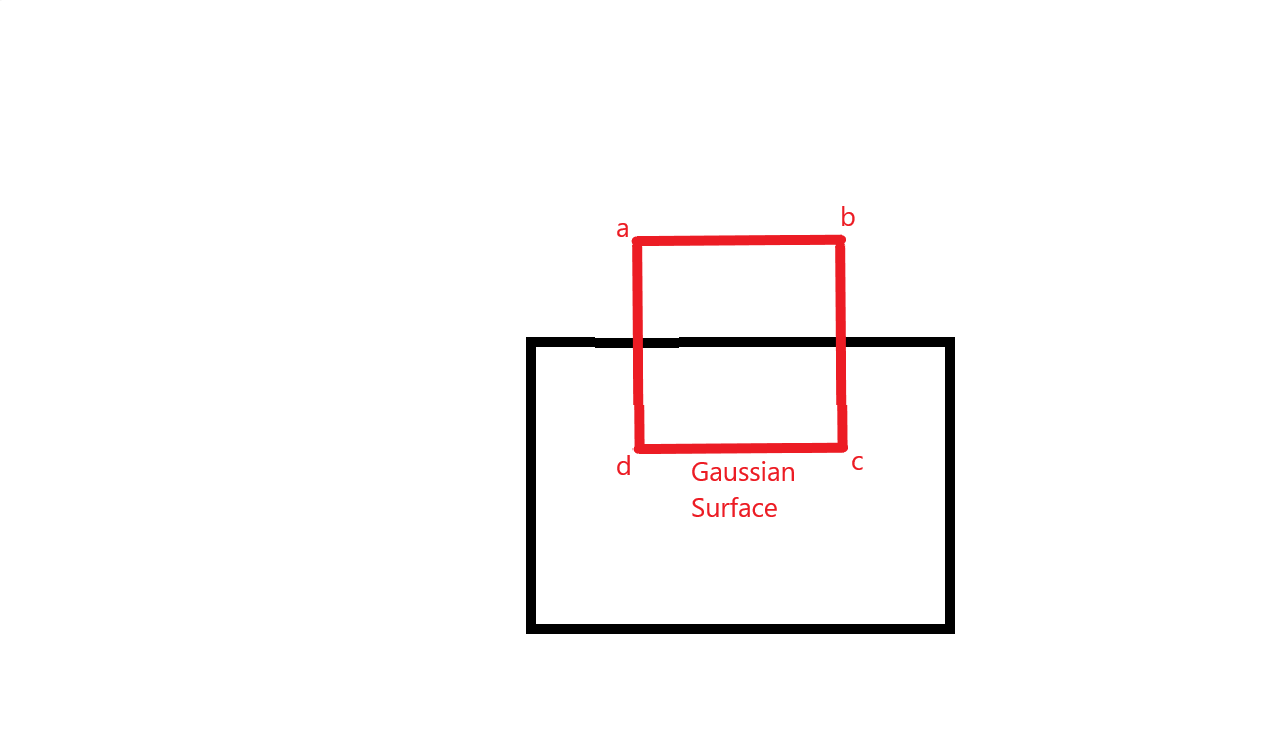
\includegraphics[width=0.4\textwidth]{Images/hollowgausssplit.png}\label{fig:f4}}
        \caption{Closed Gaussian Surface covering the inside and outside of a hollow box conductor}
    \end{figure}

    Using Gauss's Law in integral form (Reference equation \ref{eq: 1-6})
    \begin{gather*}
        \oint_S \vec{E} \cdot n da = \frac{\int_V \rho_q(x) d^3 x}{\epsilon_0}
    \end{gather*}

    Using points a-d, as shown in Figure 4\ref{fig:f4}:
    \begin{equation} \label{eq: 1-9}
        \int_{ab} \vec{E} \cdot n da + \int_{bc} \vec{E} \cdot n da + \int_{cd} \vec{E} \cdot n da + \int_{da} \vec{E} \cdot n da =
    \end{equation}

    The two lines that cross the conductor boundary cancel each other out
    \begin{equation} \label{eq: 1-10}
        \int_{bc} \vec{E} \cdot n da + \int_{da} \vec{E} \cdot n da = 0
    \end{equation}

    The line within the the conducting box will have no electric field
    \begin{equation} \label{eq: 1-11}
        \int_{cd} \vec{E} \cdot n da = 0
    \end{equation}

    Therefore:
    \begin{equation} \label{eq: 1-12}
        \int_{ab} \vec{E} \cdot n da = \frac{\int_V \rho_q(x) d^3 x}{\epsilon_0}
    \end{equation}

    If the only gaussian surface being affected is the top one, then the only charge being considered is the top surface of the conducting sphere. Shrink the conducting box to be "very" small. 
    \begin{equation} \label{eq: 1-13}
        \vec{E} A = \frac{q}{\epsilon_0}
    \end{equation}

    Define Charge per Unit Area ($\rho$)
    \begin{equation} \label{eq: 1-14}
        \rho = \frac{q}{A}
    \end{equation}

    Isolate E
    \begin{equation} \label{eq: 1-15}
        E = \frac{\rho}{\epsilon_0}
    \end{equation}

\newpage
\section{Textbook Question 1.2} \label{section2}
    \underline{Question: }
    \newline The Dirac delta function in three dimensions can be taken as the improper limit as $\alpha \rightarrow 0$ of the Gaussian function
    \begin{gather*}
        D(\alpha; x, y, z) = (2 \pi)^{-\frac{3}{2}} \alpha^{-3} e^{-\frac{1}{2 \alpha^2} (x^2 + y^2 + z^2}
    \end{gather*}
    Consider a general orthogonal coordinate system specified by the surfaces $u = constant$, $v = constant$, and $w = constant$ with length elements $\frac{du}{U}$, $\frac{dv}{V}$, and $\frac{dw}{W}$ in the three perpendicular directions. Show that
    \begin{gather*}
        \delta(x-x') = \delta(u-u') \delta(v-v') \delta(w-w') \cdot UVW
    \end{gather*}
    by considering the limit of the Gaussian above. Note that as $\alpha \rightarrow 0$ only the infintesimal length element need be used for the distance between the points in the exponent.

    Using the Dirac Delta property
    \begin{equation} \label{eq: 2-1}
        \int_{-\inf}^{\inf} \int_{-\inf}^{\inf} \int_{-\inf}^{\inf} \delta(x) \delta(y) \delta(z) dx dy dz = 1
    \end{equation}

    Use the gaussian equation instead of deltas
    \begin{equation} \label{eq: 2-2}
        \int_{-\inf}^{\inf} \int_{-\inf}^{\inf} \int_{-\inf}^{\inf} \lim_{\alpha \rightarrow 0} D(\alpha; x, y, z) dx dy dz = 1
    \end{equation}

    Use length elements
    \begin{equation} \label{eq: 2-3}
        \int_{-\inf}^{\inf} \int_{-\inf}^{\inf} \int_{-\inf}^{\inf} \lim_{\alpha \rightarrow 0} D(\alpha; x, y, z \rightarrow u, v, w) \frac{du}{U} \frac{dv}{V} \frac{dw}{W} = 1
    \end{equation}

    Compare
    \begin{equation} \label{eq: 2-4}
        D(\alpha; x, y, z \rightarrow u, v, w) \frac{du}{U} \frac{dv}{V} \frac{dw}{W} = \delta(x-x') = \delta(u-u') \delta(v-v') \delta(w-w')
    \end{equation}

    Isolate D
    \begin{equation} \label{eq: 2-5}
        D(\alpha; x, y, z \rightarrow u, v, w) = \delta(x-x') = \delta(u-u') \delta(v-v') \delta(w-w') UVW
    \end{equation}

    By definition
    $D(\alpha; x, y, z \rightarrow u, v, w) = \delta(x-x')$

    Therefore;
    \begin{equation} \label{eq: 2-6}
        \boxed{\boldsymbol{\delta(x-x') = \delta(x-x') = \delta(u-u') \delta(v-v') \delta(w-w') UVW}}
    \end{equation}

\newpage
\section{Textbook Question 3} \label{section3}
    \underline{Question: }
    \newline Using Dirac delta functions in the appropriate coordinates, express the following charge distributions as three-dimensional charge densities $\rho(x)$
    \begin{itemize}
        \item In spherical coordinates, a charge Q uniformly distributed over a spherical shell of radius R.
        \item In cylindrical coordinates, a charge A per unit length uniformly distributed over a cylindrical surface of radius b.
        \item In cylindrical coordinates, a charge Q spread uniformly over a flat circular disc of negligible thickness and radius R.
        \item The same as part (c), but using spherical coordinates.
    \end{itemize}

    \underline{Question 3, Section 1 Answer: }
    \newline \newline For a uniformally charged ($Q$) shell with radius $r=R$ and a normalization constant ($A$), the charge density is
    \begin{equation} \label{eq:3-1}
        \rho(x) = A \delta(r-R)
    \end{equation}

    Integrate the density over the volume of the shell to get Q
    \begin{equation} \label{eq:3-2}
        Q = \int \int \int \rho(x) dx = \int_0^\pi \int_0^{2 \pi} \int_0^{\inf} A \delta(r-R) (r^2 sin(\theta)) dr d\phi d\theta
    \end{equation}
    \begin{gather*}
        Q = A (2) (2 \pi) (R^2)
    \end{gather*}

    Isolate A
    \begin{equation} \label{eq:3-3}
        A = \frac{Q}{4 \pi R^2}
    \end{equation}

    Making the charge density 
    \begin{equation} \label{eq:3-4}
        \boxed{\boldsymbol{\rho(x) = \frac{Q}{4 \pi R^2} \delta(r-R)}}
    \end{equation}

    \underline{Question 3, Section 2 Answer: }
    \newline \newline For a uniformly charged ($\lambda$) cylindrical surface with radius $r=b$ and a normalization constant ($A$), the charge density is
    \begin{equation} \label{eq:3-1}
        \rho(x) = A \delta(r-b)
    \end{equation}

    Integrate the density over the volume to get $\lambda$
    \begin{equation} \label{eq:3-2}
        \lambda = \int \int \int \rho(x) dx = \int_0^1 \int_0^{2 \pi} \int_0^{\inf} A \delta(r-b) (r dr d\phi dz)
    \end{equation}
    \begin{gather*}
        Q = A (1) (2 \pi) (b)
    \end{gather*}

    Isolate A
    \begin{equation} \label{eq:3-3}
        A = \frac{\lambda}{2 \pi b}
    \end{equation}

    Making the charge density 
    \begin{equation} \label{eq:3-4}
        \boxed{\boldsymbol{\rho(x) = \frac{\lambda}{2 \pi b} \delta(r-b)}}
    \end{equation}
    
    \underline{Question 3, Section 3 Answer: }
    \newline \newline For a uniformly charged ($Q$) circular disk with radius from $r=0$ to $r=R$ and a normalization constant ($A$), the charge density is
    \begin{equation} \label{eq:3-1}
        \rho(x) = A (H(r-0) - H(r-R)) \delta(z)
    \end{equation}
    
    Integrate the density over the volume to get $Q$
    \begin{equation} \label{eq:3-2}
        Q = \int \int \int \rho(x) dx = \int_{-1}^1 \int_0^{2 \pi} \int_0^{\inf} A (H(r-0) - H(r-R)) \delta(z) (r dr d\phi dz)
    \end{equation}  
    \begin{gather*}
        Q = A (1) (2 \pi) (\frac{R^2}{2})
    \end{gather*}

    Isolate A
    \begin{equation} \label{eq:3-3}
        A = \frac{Q}{\pi R^2}
    \end{equation}

    Making the charge density 
    \begin{equation} \label{eq:3-4}
        \boxed{\boldsymbol{\rho(x) = \frac{Q (H(r-0) - H(r-R)) \delta(z)}{\pi R^2}}}
    \end{equation}

    \underline{Question 3, Section 4 Answer: }
    \newline \newline For a uniformly charged ($Q$) circular disk with radius from $r=0$ to $r=R$ and a normalization constant ($A$), the charge density is
    \begin{equation} \label{eq:3-1}
        \rho(x) = A (H(r-0) - H(r-R)) \delta(\theta - \frac{\pi}{2})
    \end{equation}

    Integrate the density over the volume to get $Q$
    \begin{equation} \label{eq:3-2}
        Q = \int \int \int \rho(x) dx 
    \end{equation}  
    \begin{gather*}
        Q = \int_0^{\pi} \int_0^{2 \pi} \int_0^{\inf} A (H(r-0) - H(r-R)) \delta(\theta - \frac{\pi}{2}) (r^2 sin(\theta) dr d\phi d\theta)
        \\ = A (1) (2 \pi) (\frac{R^3}{3})
    \end{gather*}

    Isolate A
    \begin{equation} \label{eq:3-3}
        A = \frac{3Q}{2 \pi R^3}
    \end{equation}

    Making the charge density 
    \begin{equation} \label{eq:3-4}
        \boxed{\boldsymbol{\rho(x) = \frac{3 Q (H(r-0) - H(r-R)) \delta(\theta - \frac{\pi}{2})}{2 \pi R^3}}}
    \end{equation}

\newpage
\section{Textbook Question 1.4} \label{section4}
    \underline{Question: }
    \newline Each of three charged spheres of radius a, one conducting, one having a uniform charge density within its volume, and one having a spherically symmetric charge density that varies radially as $r^n$ ($n > —3$), has a total charge Q. Use Gauss’s theorem to obtain the electric fields both inside and outside each sphere. Sketch the behavior of the fields as a function of radius for the first two spheres, and for the third with $n = - 2 + 2$.

    I hate that the question notes the radius of each sphere to be $a$ when we use $R$ typically. Also, $da$ is area, so that would be confusing. The below formulations will use $R$ as the radius of the sphere.

    \underline{Question 4, Section 1 Answer: }
    \newline \newline Using Gauss Law in integral form (Reference equation \ref{eq: 1-6})
    \begin{equation}
        \oint_S \vec{E} \cdot n da = \frac{\int_V \rho_q(x) d^3 x}{\epsilon_0}        
    \end{equation}

    The sphere is symmetrical, so $\vec{E}$ is constant
    \begin{equation} \label{eq: 4-1}
        \vec{E} \oint_S da = \frac{\int_V \rho_q(x) d^3 x}{\epsilon_0}         
    \end{equation}

    If the sphere is "very small" then it acts like a point charge
    \begin{equation} \label{eq: 4-2}
        \vec{E} \oint_S da = \frac{Q}{\epsilon_0}         
    \end{equation}

    Integrate
    \begin{equation} \label{eq: 4-3}
        E 4 \pi r^2 = \frac{Q}{\epsilon_0}
    \end{equation}

    Isolate E to get the electric field outside of the sphere
    \begin{equation} \label{eq: 4-4}
        \boxed{\boldsymbol{E_{outside} = \frac{Q}{4 \pi r^2 \epsilon_0}}}
    \end{equation}

    The electric field is non-existant inside of the closed surface
    \begin{equation} \label{eq: 4-5}
        E_{inside} = 0
    \end{equation}

    \underline{Question 4, Section 2 Answer: }
    \newline \newline Using Gauss Law in integral form (Reference equation \ref{eq: 1-6})
    \begin{equation}
        \oint_S \vec{E} \cdot n da = \frac{\int_V \rho_q(x) d^3 x}{\epsilon_0}        
    \end{equation}

    The sphere is symmetrical, so $\vec{E}$ is constant
    \begin{equation} \label{eq: 4-7}
        \vec{E} \oint_S da = \frac{\int_V \rho_q(x) d^3 x}{\epsilon_0}         
    \end{equation}

    The charge density ($\rho$) takes into account the uniform charge density within the sphere's volume ($Q$) and the charge on the surface
    \begin{equation} \label{eq: 4-8}
        \rho = (\frac{Q}{\frac{4}{3} \pi R^3}) (\frac{4}{3} \pi r^3)
    \end{equation}

    Reduce algebraically, plug into reduced gauss law, and integrate
    \begin{equation} \label{eq: 4-9}
        E 4 \pi r^2 = \frac{Q r^3}{\epsilon_0 R^3}
    \end{equation}

    Isolate $E$
    \begin{equation} \label{eq: 4-10}
        \boxed{\boldsymbol{E = \frac{Q r}{4 \pi \epsilon_0 R^3}}}
    \end{equation}

    Since the inside of the conducting sphere is shielded from electric fields outside of the inner wall, we will only consider the charge density in the volume of the sphere. 
    \begin{equation} \label{eq: 4-11}
        \rho = (\frac{Q}{\frac{4}{3} \pi R^3})
    \end{equation}

    Reduce algebraically, plug into reduced gauss law, and integrate
    \begin{equation} \label{eq: 4-12}
        E 4 \pi r^2 = \frac{3 Q r^3}{4 \epsilon_0 \pi R^3}
    \end{equation}

    Isolate $E$
    \begin{equation} \label{eq: 4-13}
        \boxed{\boldsymbol{E = \frac{3 Q}{\epsilon_0 \pi^2 r^2 R^3}}}
    \end{equation}

    \underline{Question 4, Section 2 Answer: }
    \newline \newline For the outside of the sphere, it has the same electric field as equation \ref{eq: 4-4}
    \begin{equation}
        \boxed{\boldsymbol{E_{outside} = \frac{Q}{4 \pi r^2 \epsilon_0}}}
    \end{equation}

    For the inside we will again begin by using Gauss Law in integral form (Reference equation \ref{eq: 1-6})
    \begin{equation}
        \oint_S \vec{E} \cdot n da = \frac{\int_V \rho_q(x) d^3 x}{\epsilon_0}        
    \end{equation}

    The sphere is symmetrical, so $\vec{E}$ is constant (Reference equation \ref{eq: 4-7})
    \begin{equation}
        \vec{E} \oint_S da = \frac{\int_V \rho_q(x) d^3 x}{\epsilon_0}         
    \end{equation}

    The charge density is not constant, but varies as $r^n$.
    \begin{equation} \label{eq: 4-14}
        \rho = A r^n
    \end{equation}

    Integrate the charge density over the whole sphere to find $A$, the constant
    \begin{equation} \label{eq: 4-15}
        \int_0^{2 \pi} \int_0^{\pi} \int_0^R A r^n r^2 sin(\theta) d\theta d\phi dr = Q
    \end{equation}

    Isolate A
    \begin{equation} \label{eq: 4-16}
        A = \frac{Q}{4 \pi (\frac{R^{n+3}}{n+3})}
    \end{equation}

    Plug into gauss and convert coordinates to polar
    \begin{equation} \label{eq: 4-17}
        \vec{E} \oint_S da = \frac{\int_0^{2 \pi} \int_0^{\pi} \int_0^R \frac{Q}{4 \pi (\frac{R^{n+3}}{n+3})} r^n r^2 sin(\theta) d\theta d\phi dr}{\epsilon_0}         
    \end{equation}

    Integrate
    \begin{equation} \label{eq: 4-18}
        E 4 \pi r^2 = \frac{Q r^{n+3}}{R^{n+3} \epsilon_0}
    \end{equation}

    Isolate E
    \begin{equation} \label{eq: 4-19}
        \boxed{\boldsymbol{E = \frac{Q r^{n+3}}{4 \pi \epsilon_0 r^2 R^{n+3}}}}
    \end{equation}

    for $n=-2$
    \begin{equation} \label{eq: 4-20}
        \boxed{\boldsymbol{E = \frac{Q}{4 \pi \epsilon_0 r R}}}
    \end{equation}

    for $n=+2$
    \begin{equation} \label{eq: 4-20}
        \boxed{\boldsymbol{E = \frac{Q r^3}{4 \pi \epsilon_0 R^5}}}
    \end{equation}

\newpage
\section{Textbook Question 5} \label{section5}
    \underline{Question: }
    \newline The time-averaged potential of a neutral hydrogen atom is given by 
    \begin{equation}
        \Phi = \frac{q}{4 \pi \epsilon_0} \frac{e^{\alpha r}}{r} (1 + \frac{\alpha r}{2})
    \end{equation}
    where $q$ is the magnitude of the electronic charge, and $\alpha^{-1} = \frac{a_0}{2}$, $a_0$ being the Bohr radius. Find the distribution of charge (both continuous and discrete) that will give this potential and interpret your result physically.

    \underline{Question 5, Section 1 Answer: }
    \newline \newline From Poisson's equation and gauss's law in integration form
    \begin{equation} \label{eq: 5-1}
        \nabla^2 \Phi = - \frac{\rho}{\epsilon_0}
    \end{equation}

    Expand the gradient into its individual spherical coordinates
    \begin{equation} \label{ea: 5-2}
        \frac{1}{r^2} \frac{\partial}{\partial r} (r^2 \frac{\partial \Phi}{\partial r}) + \frac{1}{r^2 sin(\theta)} \frac{\partial}{\partial \theta} (sin(\theta) \frac{\partial \Phi}{\partial \theta}) + \frac{1}{r^2 sin^2(\theta)} \frac{\partial^2 \Phi}{\partial \phi^2} = - \frac{\rho}{\epsilon_0}
    \end{equation}

    The potential is spherically symmetric, so $\frac{\partial}{\partial \theta} = 0$ and $\frac{\partial^2 \Phi}{\partial \phi^2} = 0$

    The reduced poisson equation is
    \begin{equation} \label{eq: 5-3}
        \frac{1}{r^2} \frac{\partial}{\partial r} (r^2 \frac{\partial \Phi}{\partial r}) = - \frac{\rho}{\epsilon_0}
    \end{equation}

    Insert given formula for $\Phi$
    \begin{equation} \label{eq: 5-4}
        \frac{1}{r^2} \frac{\partial}{\partial r} (r^2 \frac{\partial (\frac{q}{4 \pi \epsilon_0} \frac{e^{\alpha r}}{r} (1 + \frac{\alpha r}{2}))}{\partial r}) = - \frac{\rho}{\epsilon_0}
    \end{equation}

    Reduce and isolate $q$
    \begin{equation} \label{eq: 5-5}
        \rho = \frac{- q \alpha^3 e^{-\alpha r}}{8 \pi} - \frac{e^{-\alpha r} q}{4 \pi r^2} \frac{\partial}{\partial r} (r^2 \frac{\partial}{\partial r} \frac{1}{r})
    \end{equation}

    If $r=0$ then this equation contains singularities, infinities, and is non-physical.
    We will consider the same equation for two cases ($r \approx 0$ and $r > 0$)
    For $r \approx 0$, $e^{\alpha r} \approx 1$ so 
    \begin{equation} \label{eq: 5-6}
        \rho = \frac{-q \alpha^3}{8 \pi} - \frac{q}{r \pi} \frac{1}{r^2} \frac{\partial}{\partial r} (r^2 \frac{\partial}{\partial r} \frac{1}{r})
    \end{equation}

    Using the delta relation
    \begin{equation} \label{eq: 5-7}
        \nabla^2 \frac{1}{r} = -4 \pi \delta(r)
    \end{equation}

    Expand the gradient into its individual spherical coordinates
    \begin{equation} \label{eq: 5-8}
        \frac{1}{r^2} \frac{\partial}{\partial r} (r^2 \frac{\partial}{\partial r} \frac{1}{r}) = - 4 \pi \delta(r)
    \end{equation}

    Substitute equation \ref{eq: 5-8} in equation \ref{eq: 5-6}
    \begin{equation} \label{eq: 5-9}
        \rho = \frac{-q \alpha^3}{8 \pi} - \frac{q}{r \pi} (- 4 \pi \delta(r))
    \end{equation}

    Reduce 
    \begin{equation} \label{eq: 5-10}
        \rho = \frac{-q \alpha^3}{8 \pi} + q \delta(r)
    \end{equation}

    For $r > 0$ evaluate derivatives normally
    \begin{equation} \label{eq: 5-11}
        \rho = \frac{-q \alpha^3}{8 \pi} e^{- \alpha r}
    \end{equation}

    The equations can be combined because if $r \approx 0$ this general equation reduces to it "case" equation
    \begin{equation} \label{eq: 5-12}
        \boxed{\boldsymbol{\rho = \frac{-q \alpha^3}{8 \pi} e^{- \alpha r}+ q \delta(r)}}
    \end{equation}

\newpage
\section{Custom Notes Question} \label{section6}
    \underline{Question: }
    \newline \newline Separation of Variables: Laplace Equation in Spherical Coordinates

    We begin with the laplace equation
    \begin{equation} \label{eq: 6-1}
        \nabla^2 \Phi = 0
    \end{equation}

    Expanding the nabla to spherical polar coordinates
    \begin{equation} \label{eq: 6-2}
        \frac{1}{r} \frac{\partial^2}{\partial r^2} (r \Phi) + \frac{1}{r^2 sin(\theta)} \frac{\partial}{\partial \theta} (sin(\theta) \frac{\partial \Phi}{\partial \theta}) + \frac{1}{r^2 sin^2(\theta)} \frac{\partial^2 \Phi}{\partial \phi^2} = 0
    \end{equation}

    Use the method of separation by trying a solution of the form
    \begin{equation} \label{eq: 6-3}
        \Phi(r,\theta, \Phi) = \frac{R(r)}{r} P(\theta) Q(\phi)
    \end{equation}

    Substitute equation \ref{eq: 6-3} into equation \ref{eq: 6-2}
    \begin{gather*}
        \frac{1}{r} \frac{\partial^2}{\partial r^2} (r \frac{R(r)}{r} P(\theta) Q(\phi)) 
        \\ + \frac{1}{r^2 sin(\theta)} \frac{\partial}{\partial \theta} (sin(\theta) \frac{\partial \frac{R(r)}{r} P(\theta) Q(\phi)}{\partial \theta}) 
        \\ + \frac{1}{r^2 sin^2(\theta)} \frac{\partial^2 \frac{R(r)}{r} P(\theta) Q(\phi)}{\partial \phi^2} = 0
    \end{gather*}

    Reduce algebraically
    \begin{gather*}
        P(\theta)Q(\phi) \frac{1}{r} \frac{\partial^2 R(r)}{\partial r^2} 
        \\ + \frac{R(r)}{r} Q(\phi) \frac{1}{r^2 sin(\theta)} \frac{\partial}{\partial \theta} (sin(\theta) \frac{\partial P(\theta)}{\partial \theta}) 
        \\ + \frac{R(r)}{r} P(\theta) \frac{1}{r^2 sin^2(\theta)} \frac{\partial^2 Q(\phi)}{\partial \phi^2} = 0
    \end{gather*}

    Reduce by multiplying the entire equation by $\frac{r^3 sin^2(\theta)}{R(r)P(\theta)Q(\phi)}$
    \begin{equation} \label{eq: 6-6}
        \frac{r^2sin^2(\theta)}{R(r)} \frac{d^2 R(r)}{dr^2} + \frac{sin(\theta)}{P(\theta)} \frac{d}{d \theta} (sin(\theta) \frac{d P(\theta)}{d \theta} + \frac{1}{Q(\phi)} \frac{d^2 Q(\phi)}{d \phi^2} = 0
    \end{equation}

    A singular term is only dependent on 1 coordinate
    \begin{equation} \label{eq: 6-7}
        -m^2 = \frac{1}{Q(\phi)} \frac{d^2 Q(\phi)}{d \phi^2}
    \end{equation}

    Rearrange equation to be in differential form
    \begin{equation} \label{eq: 6-8}
        \frac{d^2 Q(\phi)}{d \phi^2} = -m^2 Q(\phi)
    \end{equation}

    General solution for $Q(\phi)$
    \begin{equation} \label{eq: 6-9}
        Q(\phi) = A_m e^{im\phi} + B_m e^{im\phi}
    \end{equation}

    Substitute equation \ref{eq: 6-7} into equation \ref{eq: 6-6}
    \begin{equation} \label{eq: 6-10}
        \frac{r^2sin^2(\theta)}{R(r)} \frac{d^2 R(r)}{dr^2} + \frac{sin(\theta)}{P(\theta)} \frac{d}{d \theta} (sin(\theta) \frac{d P(\theta)}{d \theta} -m^2 = 0
    \end{equation}

    Reduce by multiplying the entire equation by $sin^2(\theta)$
    \begin{equation} \label{eq: 6-11}
        \frac{r^2}{R(r)} \frac{d^2 R(r)}{dr^2} + \frac{1}{sin(\theta) P(\theta)} \frac{d}{d \theta} (sin(\theta) \frac{d P(\theta)}{d \theta} - \frac{m^2}{sin^2(\theta)} = 0
    \end{equation}

    Two terms are dependent on 1 coordinate
    \begin{equation} \label{eq: 6-12}
        -l(l+1) = \frac{1}{sin(\theta) P(\theta)} \frac{d}{d \theta} (sin(\theta) \frac{d P(\theta)}{d \theta} - \frac{m^2}{sin^2(\theta)}
    \end{equation}

    Substitute equation \ref{eq: 6-12} into equation \ref{eq: 6-11}
    \begin{equation} \label{eq: 6-14}
        \frac{r^2}{R(r)} \frac{d^2 R(r)}{dr^2}-l(l+1) = 0
    \end{equation}

    Rearrange equation to be in differential form
    \begin{equation} \label{eq: 6-15}
        \frac{d^2 R(r)}{dr^2} = -l(l+1)\frac{R(r)}{r^2} 
    \end{equation}

    General solution for $R(r)$
    \begin{equation} \label{6-16}
        R(r) = A_l r^{l+1} + B_l r^{-l}
    \end{equation}





















    

\begin{comment}

    \begin{equation} \label{eq:1-1}
        a=a  
    \end{equation}
\section{Template Functions} \label{section100}

\subsection{Equations} \label{subsection100-1}
    
    %% Referencialable Equation
    \begin{equation} \label{eq:100-1-1}
        a \cdot (b \cross c) = b \cdot (c \cross a) = c \cdot (a \cross b   
    \end{equation}

    %% Just Centered
    \begin{gather*}
        var=-\sigma * n_1 * \Gamma dx
    \end{gather*}

    var = $Q_{DT}=2\times10^{-12}$

\subsection{Organization}
$\boxed{\boldsymbol{ayo}}$

\subsection{Greek}
    \begin{gather*}
        \lambda, \sigma, \tau
    \end{gather*}

\subsection{Math Symbols}
    \begin{gather*}
        \int, \infty, \frac{a}{b}, \vec{v}, \geq, \approx
    \end{gather*}

\subsection{Images}
    \begin{figure}[H]
        \centering
        {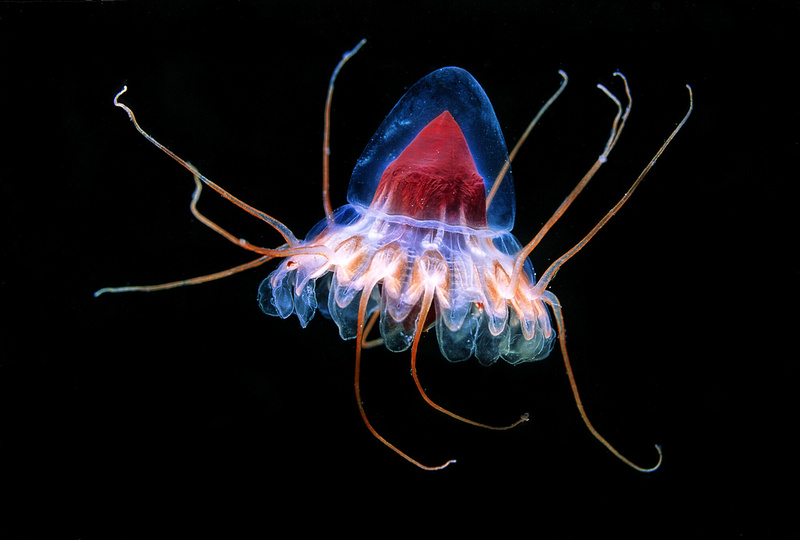
\includegraphics[width=0.4\textwidth]{Images/Template/Jelly1.jpg}\label{fig:f2}}
        \caption{Jelly1}
    \end{figure}
    \begin{figure}[H]
        \centering
        \subfloat[Jelly2]{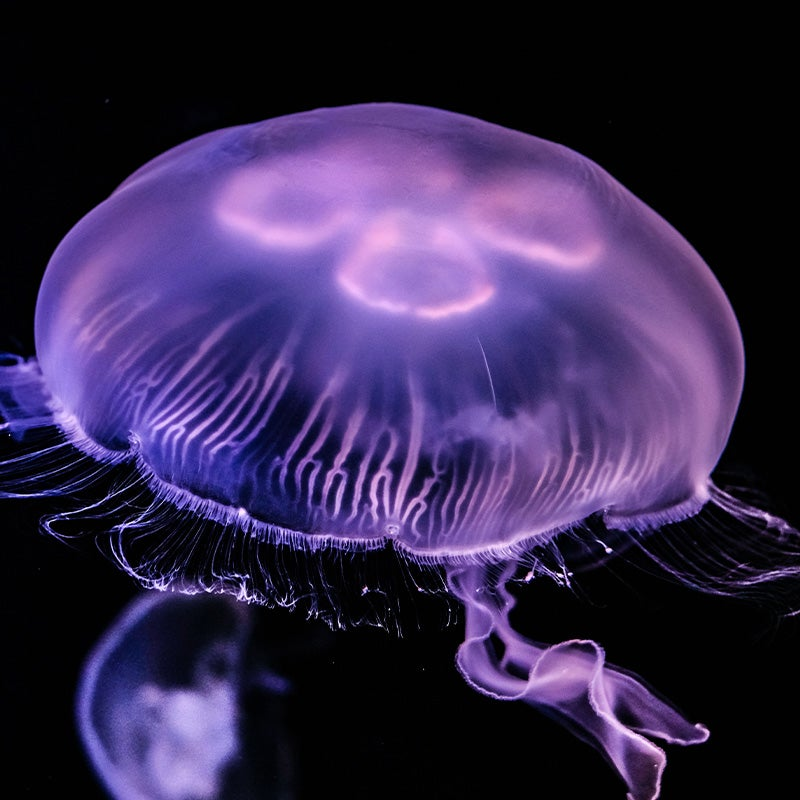
\includegraphics[width=0.3\textwidth]{Images/Template/Jelly2.jpg}\label{fig:f1}}
        \hfill
        \subfloat[Jelly3]{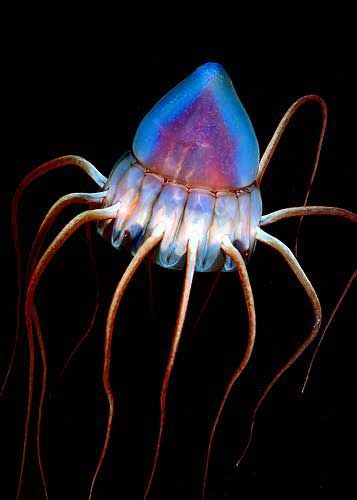
\includegraphics[width=0.3\textwidth]{Images/Template/Jelly3.jpg}\label{fig:f2}}
        \hfill
        \subfloat[Jelly4]{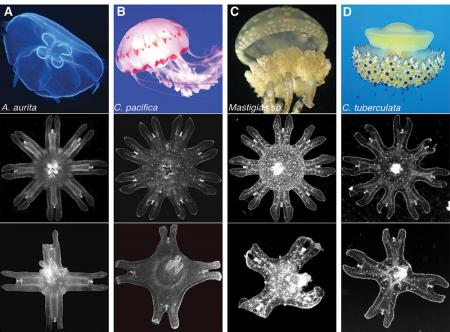
\includegraphics[width=0.3\textwidth]{Images/Template/Jelly4.jpg}\label{fig:f3}}
    \end{figure}

\subsection{Overleaf Functions}
    %% Comment

    
    \begin{gather*}
        var = a \\ 
        var = b \\
        var = c
    \end{gather*}

    %% Matrix

    \begin{pmatrix}
        $\psi_1$
        \\ $\psi_2$
        \\ $\psi_3$
    \end{pmatrix}    
    
    
    $\anti{\psi}$

    \cite{GreekLetters}
\end{comment}




\newpage
\printbibliography
\end{document}
